%
% Main thesis LaTeX file. We use the REPORT style format
% instead of article for most technical papers
%
%
\documentclass[11pt,fleqn]{article}

%%%%%%%%%%%%%%%%%%%%%%%%%%%%%%%%%%%%%%%%%%%%%%%%%%%%%%%%%%%%%%%%%%%%
%
% list the set of packages we use for various aspects of 
% the thesis format
%
\usepackage{layout}
\usepackage[utf8]{inputenc}
\usepackage{setspace}

\usepackage{subfigure}
\usepackage{epsfig}
\usepackage{float}
\usepackage{floatflt}
\usepackage{listings}
\usepackage{palatino}
\usepackage{verbatim}
\usepackage{footnpag}
\usepackage{caption}
\usepackage[mathcal, mathbf]{euler}
\usepackage{amsmath}
\usepackage{amstext}
\usepackage{color}
\usepackage{xcolor}
\usepackage{graphicx}


%%%%%%%%%%%%%%%%%%%%%%%%%%%%%%%%%%%%%%%%%%%%%%%%%%%%%%%%%%%%%%%%%%%%
%
% include two local LaTeX source files that establish the
% thesis layout and the set of additional commands we find
% useful for creating the text.
%
\input{layout}
\input{newcommands}
\input{outline_support}


\newcommand{\Organization}{School of Computer Engineering}

\title{CE3001 Lab1. Arithmetic Logic Unit(ALU)}

\author{
  Lu Shengliang \\
  SLU001\\
  \Organization{} \\
  \vspace*{-10mm} \\
  Nanyang Technological University \\
  \vspace*{-10mm} \\
  SLU001@e.ntu.edu.sg
}

%
% This begins the actual lab report
%
\renewcommand{\OutlineLevel}{2}

\begin{document}

\maketitle

\begin{abstract}
\ls{1}
An Arithmetic Logic Unit(ALU) is a circuit that does arithmetic, such as addition, subtraction, bit‐wise AND, bit‐wise OR, etc. The ALU is entirely combinational logic implemented in Verilog, with no storage or sequential operations.
\ls{1.2}
\end{abstract}

\ls{1.2}


\section{Introduction}

\label{sec:intro}

%=====================================================================
\subsection{Description of ALU {\em Operations}} 

The eight computation types of ALU in this lab report are: \emph{Addition}, \emph{Subtraction}, \emph{Logical AND}, \emph{Logical OR}, \emph{Shift left logical}, \emph{Shift right logical}, \emph{Shift right arithmetic} and \emph{Rotate left}. The operations of ALU instructions are Described in the table below.
\begin{table}
  \begin{tabular}{| c | c | c | l |}
    \hline
    \textbf{Operation} & \textbf{value} & \textbf{Equation} & \textbf{Description}\\ \hline
    ADD & 000 & A + B & Addition A + B in 2's Complement format\\ \hline
    SUB & 001 & A - B & Subtraction A - B in 2's Complement format\\ \hline
    AND & 010 & A \&{} B & Logical(bit‐wise) AND of A, B\\ \hline
    OR & 011 & A \textbar{} B & Logical(bit-wise) AND of A,B\\ \hline
    SLL & 100 & A \textless \textless{} Imm & Shift left logical\\ \hline
    SRL & 101 & A \textgreater \textgreater{} Imm & Shift right logical\\ \hline
    SRA & 110 & A \textgreater \textgreater{} Imm(MSB shifted in) & shift right arithmetic\\ \hline
    RL & 111 & A rot Imm & Rotate left\\
    \hline
  \end{tabular}
  
  \begin{tablenotes}
    \emph{Note}: The interface to the ALU consists of \emph{A, B, op, Imm and out}. The information is listed in the table below.
  \end{tablenotes}
  \caption{Description of ALU Operations}
\end{table}


\begin{table}
  \begin{tabular}{| c | l | r | l | c |}
    \hline
    \textbf{Port Name} & \textbf{Port Direction} & \textbf{size} & \textbf{Description}\\ \hline \hline
    A & Input & 16-bit & First operand\\ \hline
    B & Input & 16-bit & Second operand\\ \hline
    op & Input & 3-bit & Specify operation to be performed\\ \hline
    Imm & Input & 4-bit & Second amount for SLL, SRL, SRA and RL\\ \hline
    Out & Output & 16-bit & Output of the operation\\
    \hline
  \end{tabular}
  \caption{Port List Specification}
\end{table}
     
%=====================================================================


%=====================================================================

%=====================================================================
\subsection{Structure of the rest of the paper}
The rest of the paper first describes the Verilog implementation of ALU in \emph{Section \ref{sec:impl}}. \emph{Section \ref{sec:eval}} presents the experimental results using testbench, which valid the functions of our ALU. \emph{Section \ref{sec:concl}} presents our conclusions and discussions.
%=====================================================================


\section{Implementation}
\label{sec:impl}

%=====================================================================
%\subsection{How to Implementation Using Verilog}
%The first 7 operations, ADD SUB AND OR SLL SRL and SRA, can be implemented by using Verilog arithmetic operators, logical operators, shift operators. The used operations in the code have been listed below.

\subsection{Verilog Code alu.v}
The basic operations for Verilog implementing ALU  are \emph{arithmetic operators}, \emph{logical operators}, \emph{shift operators} and \emph{concatenation}.
\lstset {
    language=Verilog,
    backgroundcolor=\color{black!5},
    basicstyle=\ttfamily\footnotesize,
    numbers=left,
    numberstyle=\tiny,
    frame=single
}
\renewcommand{\baselinestretch}{0.75}
\begin{lstlisting}
module alu(A, B, op, out, Imm);
  
  input signed [15:0] A, B;
  input [2:0] op;
  input [3:0] Imm;
  output [15:0] out;
  
  wire [3:0] i;
  reg [15:0] out;
  reg [31:0] tmp;
  
  always @(A or B or op)
    begin
      case (op)
      3'b000: out = A + B;        //ADD
      3'b001: out = A - B;        //SUB
      3'b010: out = A && B;       //AND
      3'b011: out = A || B;       //OR
      3'b100: out = A << Imm;     //SLL
      3'b101: out = A >> Imm;     //SRL
      3'b110: out = A >>> Imm;    //SRA
      3'b111:                     //RL
        begin
          tmp = {A, A} << Imm;
          out = tmp[31:16];
        end
      default: out = 16'd0;
    endcase
  end
  
endmodule
\end{lstlisting}
\end{\baselinestretch}
The implementation results will be listed in \emph{Section \ref{sec:eval}}.

\section{Evaluation}
\label{sec:eval}

%=====================================================================
\subsection{Testbench Code 1 alu\underline{ }tb.v}
\lstset {
    language=Verilog,
    backgroundcolor=\color{black!5},
    basicstyle=\ttfamily\footnotesize,
    numbers=left,
    numberstyle=\tiny,
    frame=single
}
\renewcommand{\baselinestretch}{0.75}
\begin{lstlisting}
module alu_tb;
  reg [15:0] A, B;
  reg [2:0] op;
  reg [3:0] imm;
  
  wire [15:0] out;
  
  alu alu0(.A(A), .B(B), .op(op), .out(out), .imm(imm));
  initial
    begin
      A = 16'd0; B = 16'd0; op = 3'b000; imm = 4'd0;
      #10 A = 16'h130f; B = 16'h5701; op = 3'b000;
      #10 A = 16'hfedc; B = 16'hab98; op = 3'b001;
      #10 A = 16'hcdef; B = 16'h89ab; op = 3'b010;
      #10 A = 16'hcdef; B = 16'h89ab; op = 3'b011;
      #10 A = 16'hb042; imm = 4'd1; op = 3'b100;
      #10 A = 16'hb042; imm = 4'd1; op = 3'b101;
      #10 A = 16'hb742; imm = 4'd4; op = 3'b110;
      #10 A = 16'hb742; imm = 4'd4; op = 3'b111;
      #10 finish;
    end
endmodule
\end{lstlisting}
\end{\baselinestretch}
A testbench has been designed to test the \emph{alu.v} file. A simulation function is provided by \emph{ModelSim} software, which is used to generate visualized test procedure for checking and debugging. We also use the simulation results to test the correctness of the output of \emph{alu.v}.


%=====================================================================

\begin{figure}[ht]
\centering
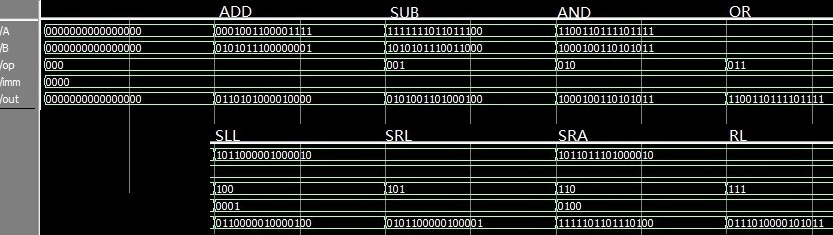
\includegraphics[width=17cm]{alu_tb.jpg}
\caption{alu Testbench Simulation Result}
\label{fig:FirstTB}
\end{figure}
%\ref{fig:FirstTB}
Simulations results are intuitive and clear for checking the current status of each inputs and outputs. Figure 1 is a simulation result shown on ModelSim software. The first testbench is using to test the functionality of alu design. According to figure 1, basic functions of alu is implemented. 

\subsection{Testbench Code 2 alu\underline{ }tb.v}
An additional testbench is assigned to test the validity of alu design, which contains more conditions for testing the implementation. The Verilog code is shown below.
\lstset {
    language=Verilog,
    backgroundcolor=\color{black!5},
    basicstyle=\ttfamily\footnotesize,
    numbers=left,
    numberstyle=\tiny,
    frame=single
}
\renewcommand{\baselinestretch}{0.75}
\begin{lstlisting}
      #10 A = 16'hfff9; B = 16'h0007; op = 3'b000;
      #10 A = 16'h0007; B = 16'hfff9; op = 3'b001;
      #10 A = 16'h89ab; B = 16'hfedc; op = 3'b010;
      #10 A = 16'h89ab; B = 16'hfedc; op = 3'b011;
      #10 A = 16'h789a; imm = 4'd15; op = 3'b100;
      #10 A = 16'h789a; imm = 4'd15; op = 3'b101;
      #10 A = 16'h8054; imm = 4'd15; op = 3'b110;
      #10 A = 16'h8754; imm = 4'd15; op = 3'b111;
\end{lstlisting}
\end{\baselinestretch}
\begin{figure}[ht]
\centering
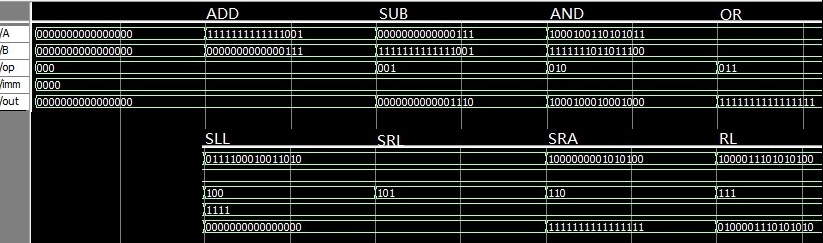
\includegraphics[width=17cm]{alu_tb2.jpg}
\caption{alu Testbench Simulations Result}
\label{fig:SecondTB}
\end{figure}
%\ref{fig:SecondTB}
For ADD operation, an overflow condition is calculated correctly.
\\
For SUB operation, an underflow condition is correct.
\\
Three 15-bit shift operations and one rotation is display properly.


\section{Conclusions and Future Work}
\label{sec:concl}
The ALU design works properly based on two testbenchs testing results.
\\ 
%=====================================================================
%\subsection{\emph{Problems} occurred in our approach}
During the Verilog implementation section, input A and B must be declared as \emph{'signed'}. Otherwise, A and B will be performed as unsigned integer by default, which will result a wrong answer after SRA operation.
\\
For this report, we use concatenation operation to implement the rotation. RL implementation methods are diverse. For instance, a for loop combined with concatenation operation can reduce the memory usage of rotation.
\\
%\subsection{Available \emph{Improvement}}
One improvement, which can be implemented, is the approaching a harder versions of ALU, by applying more efficient optimization and operations.
Another one is the combination with register files and later laboratory implementations.
%=====================================================================
\end{document}
